Le point de départ est de remarquer que \[ n^p = p^n \quad \Leftrightarrow \quad p \ln(n) = n \ln(p) \quad \Leftrightarrow \quad \frac{\ln(n)}{n}= \frac{\ln(p)}{p}.\] Ceci nous amène à étudier la fonction $f$ définie sur $]0,+\infty[$ par $f(x)=\frac{\ln(x)}{x}$. Cette fonction est dérivable sur son domaine de définition, de dérivée 
\[ f'(x)=\frac{1-\ln(x)}{x^2}.\]
On obtient le tableau de variations suivant :
\[
	\begin{tikzpicture}
		\tkzTabInit{$x$ /.8 , $f'(x)$ /.8, $f(x)$ /2}{$0$,$e$,$+\infty$}
		 \tkzTabLine{d,+,0,-,}
		\tkzTabVar{D-/ -/$-\infty$, +/ $\frac{1}{e}$ / $+\infty$,-/ $0$ /}
	\end{tikzpicture}
\]
La fonction est donc strictement croissante sur $[1,e]$, et strictement décroissante sur $[e,+\infty[$. Si les entiers naturels $(n,p)$ vérifient $f(n)=f(p)$, l'un de ces deux entiers, disons $n$, doit être dans $[1,e]$, et l'autre doit être dans $[e,+\infty[$. Or, dans $[1,e]$, il n'y a que deux entiers : $n=1$ et $n=2$. Pour $n=1$, $f(1)=0$, et la valeur nulle n'est pas prise par la fonction $f$ sur $[e,+\infty[$. Pour $n=2$, on a $f(2)=\frac{\ln(2)}{2} =f(4)$. La seule solution pour cette équation est donc $2^4=4^2$.
